% Generated by paper/build_imt_parameter_figures.py; do not hand edit.
% Q1 grid SHA-256: 1a48a6f4d5a4c6c1449f35cd7e5584b7a14d4a08f8effc2c4508497e8ef20058
\begin{figure}[tb]
\centering
\begin{minipage}[t]{.485\linewidth}
\centering
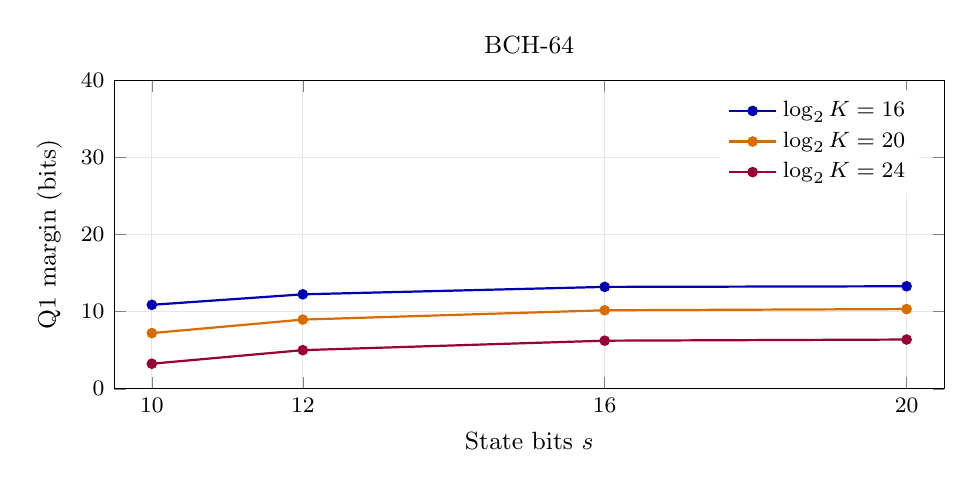
\begin{tikzpicture}
\begin{axis}[tick label style={font=\footnotesize},label style={font=\small},title style={font=\small},grid=major,grid style={black!10},legend style={font=\footnotesize,draw=none},width=\linewidth,height=5.5cm,title={BCH-64},xlabel={State bits $s$},ylabel={Q1 margin (bits)},xmin=9.5,xmax=20.5,ymin=0,ymax=40,xtick={10,12,16,20},legend pos=north east,]
\addplot[blue!70!black,thick,mark=*,mark size=1.5pt] coordinates {(10,10.8900834302) (12,12.2521826982) (16,13.2140320000) (20,13.2963998191)};
\addlegendentry{$\log_2 K=16$}
\addplot[orange!85!black,thick,mark=*,mark size=1.5pt] coordinates {(10,7.2247246256) (12,8.9772543375) (16,10.1847253778) (20,10.3403771086)};
\addlegendentry{$\log_2 K=20$}
\addplot[purple!80!black,thick,mark=*,mark size=1.5pt] coordinates {(10,3.2555009968) (12,5.0147499021) (16,6.2417426575) (20,6.3899560564)};
\addlegendentry{$\log_2 K=24$}
\end{axis}
\end{tikzpicture}
\end{minipage}
\hfill
\begin{minipage}[t]{.485\linewidth}
\centering
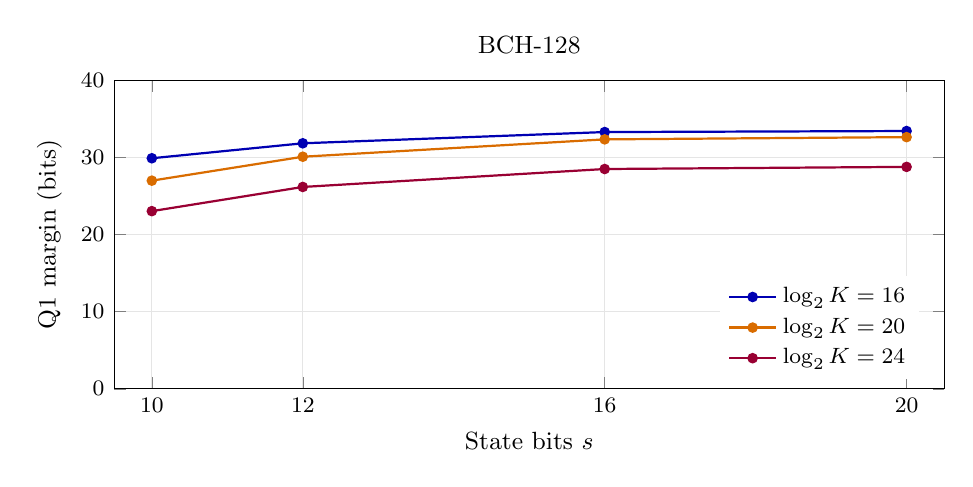
\begin{tikzpicture}
\begin{axis}[tick label style={font=\footnotesize},label style={font=\small},title style={font=\small},grid=major,grid style={black!10},legend style={font=\footnotesize,draw=none},width=\linewidth,height=5.5cm,title={BCH-128},xlabel={State bits $s$},ylabel={Q1 margin (bits)},xmin=9.5,xmax=20.5,ymin=0,ymax=40,xtick={10,12,16,20},legend pos=south east,]
\addplot[blue!70!black,thick,mark=*,mark size=1.5pt] coordinates {(10,29.8922450081) (12,31.8325429428) (16,33.2903309329) (20,33.4221485975)};
\addlegendentry{$\log_2 K=16$}
\addplot[orange!85!black,thick,mark=*,mark size=1.5pt] coordinates {(10,26.9894832727) (12,30.0911153162) (16,32.3411624023) (20,32.6317852093)};
\addlegendentry{$\log_2 K=20$}
\addplot[purple!80!black,thick,mark=*,mark size=1.5pt] coordinates {(10,23.0356798756) (12,26.1715082460) (16,28.4983268727) (20,28.7725947112)};
\addlegendentry{$\log_2 K=24$}
\end{axis}
\end{tikzpicture}
\end{minipage}
\caption{IMT state slices at three message lengths, with $t=64$ fixed.
Only the four marked states are compared at every length. Increasing
message length lowers the Q1 plateau; increasing state gives diminishing gains.}
\label{fig:finite-k-s}
\end{figure}
